\documentclass[crop,tikz]{standalone}
\usetikzlibrary{backgrounds}
\colorlet{blue}{cyan}
\tikzset{
  inverted/.style = {
    color=white,
    background rectangle/.style={fill},
    show background rectangle
  }
}
\usepackage{pgfplots}
\pgfplotsset{compat=1.18}

% Flow around a Joukowski profile with non-zero circulation.
%
% Let t(z) = a + i b and w(t) = (t + 1/t)/2. The Joukowski profile is
% given by mapping the unit circle z = e^{i\phi} to f(z) = w(t(z)).

\pgfplotsset{
  inverted/.style = {
    every axis legend/.append style={
      draw=white,
      fill=black,
      text=white
    }
  },
}

\begin{document}
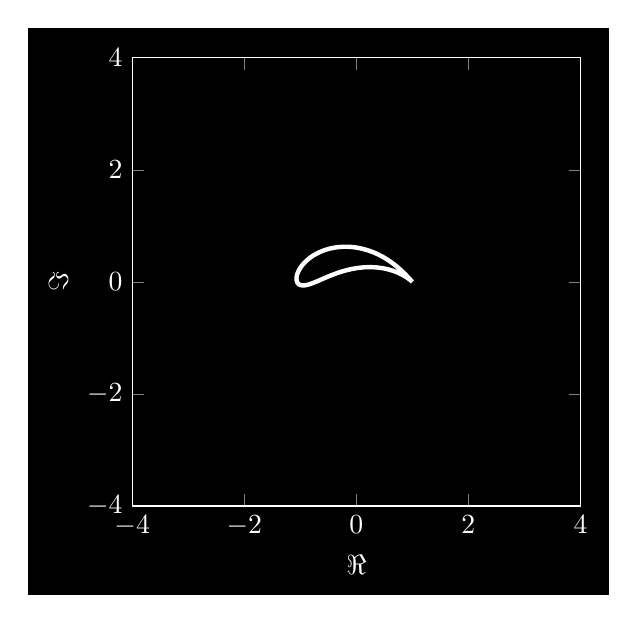
\begin{tikzpicture}[inverted,inverted]
  \pgfmathsetmacro{\remin}{-4};
  \pgfmathsetmacro{\remax}{4};
  \pgfmathsetmacro{\immin}{-4};
  \pgfmathsetmacro{\immax}{4};
  \pgfmathsetmacro{\rea}{-0.2}; % Re(a)
  \pgfmathsetmacro{\ima}{0.5}; % Im(a)
  \pgfmathsetmacro{\reb}{1.3}; % Re(b)
  \pgfmathsetmacro{\imb}{0}; % Im(b)
  \begin{axis}[inverted,
    axis equal image,
    xmin={\remin}, xmax={\remax},
    ymin={\immin}, ymax={\immax},
    xlabel={$\Re$},
    ylabel={$\Im$},
    samples=100,
    declare function = {
      nt(\p,\ra,\ia,\rb,\ib) = \ra^2 + \ia^2 + \rb^2 + \ib^2 + 2*(\ra*\rb + \ia*\ib)*cos(\p) + 2*(\ia*\rb - \ra*\ib)*sin(\p); % |a + b e^{i\phi}|^2
      rj(\p,\ra,\ia,\rb,\ib) = (\ra + \rb*cos(\p) - \ib*sin(\p))*(1 + 1/nt(\p,\ra,\ia,\rb,\ib)); % Re[w(t(e^{i\phi}))]
      ij(\p,\ra,\ia,\rb,\ib) = (\ia + \rb*sin(\p) + \ib*cos(\p))*(1 - 1/nt(\p,\ra,\ia,\rb,\ib)); % Im[w(t(e^{i\phi}))]
    },
    ]
    % Joukowski profile
    \addplot[ultra thick,domain=0:360] (
      {rj(\x,\rea,\ima,\reb,\imb)/2},
      {ij(\x,\rea,\ima,\reb,\imb)/2}
    );
  \end{axis}
\end{tikzpicture}
\end{document}
